\documentclass{article}
\usepackage{amsmath}
\usepackage{amssymb}
\usepackage{hyperref}
\usepackage{xcolor}
\usepackage{graphicx}
\usepackage{hyperref}

\title{A Modest (Tokenomics) Proposal, Version 3.4}
\date{250428}
\author{}

\begin{document}

\maketitle

\section{Goals}\label{sec:goals}
\begin{itemize}
    \item HYPR provides genuine utility to users,
    \item HYPR has long-term incentives to keep demand in long-term,
    \item HYPR allows user to participate in useful DAO governance.
\end{itemize}

\section{Voting Power}\label{sec:votingpower}

The voting power of a wallet depends on two parameters: $n$, the number of uHYPR tokens locked (there are $10^{18}$ uHYPR in one HYPR), and $t$, the remaining period tokens are locked for (in weeks).
Token supply is denoted $S$ (it is $10^9$).
Max lock time is denoted $T$ (it is some small single-digit number of years).
The voting power of a wallet is denoted $V(n, t)$.
\begin{equation}
V(n, t) = (n/a - n^2/b) \cdot (t/c - t^2/d)
\end{equation}

The parameters $a$, $b$, $c$, $d$, all greater than or equal to $0$, are chosen such that voting power is a strictly monotonically-increasing function of $n$ and $t$ (i.e. it only ever increases as $n$ and $t$ increase).
This leads to the following requirements for the parameters:
\begin{equation}\label{eq:parameters-extremum}
\begin{aligned}
1/a &\geq 2 n_m / b\\
1/c &\geq 2 T / d
\end{aligned}
\end{equation}
where $n_m$ is the maximum number of tokens that a single wallet can lock.
$n_m$ can reasonably be set to $S$.
The parameters are written as denominators to match the implementation (which is integer-, not real-number-based).

\begin{figure}[h]
    \centering
    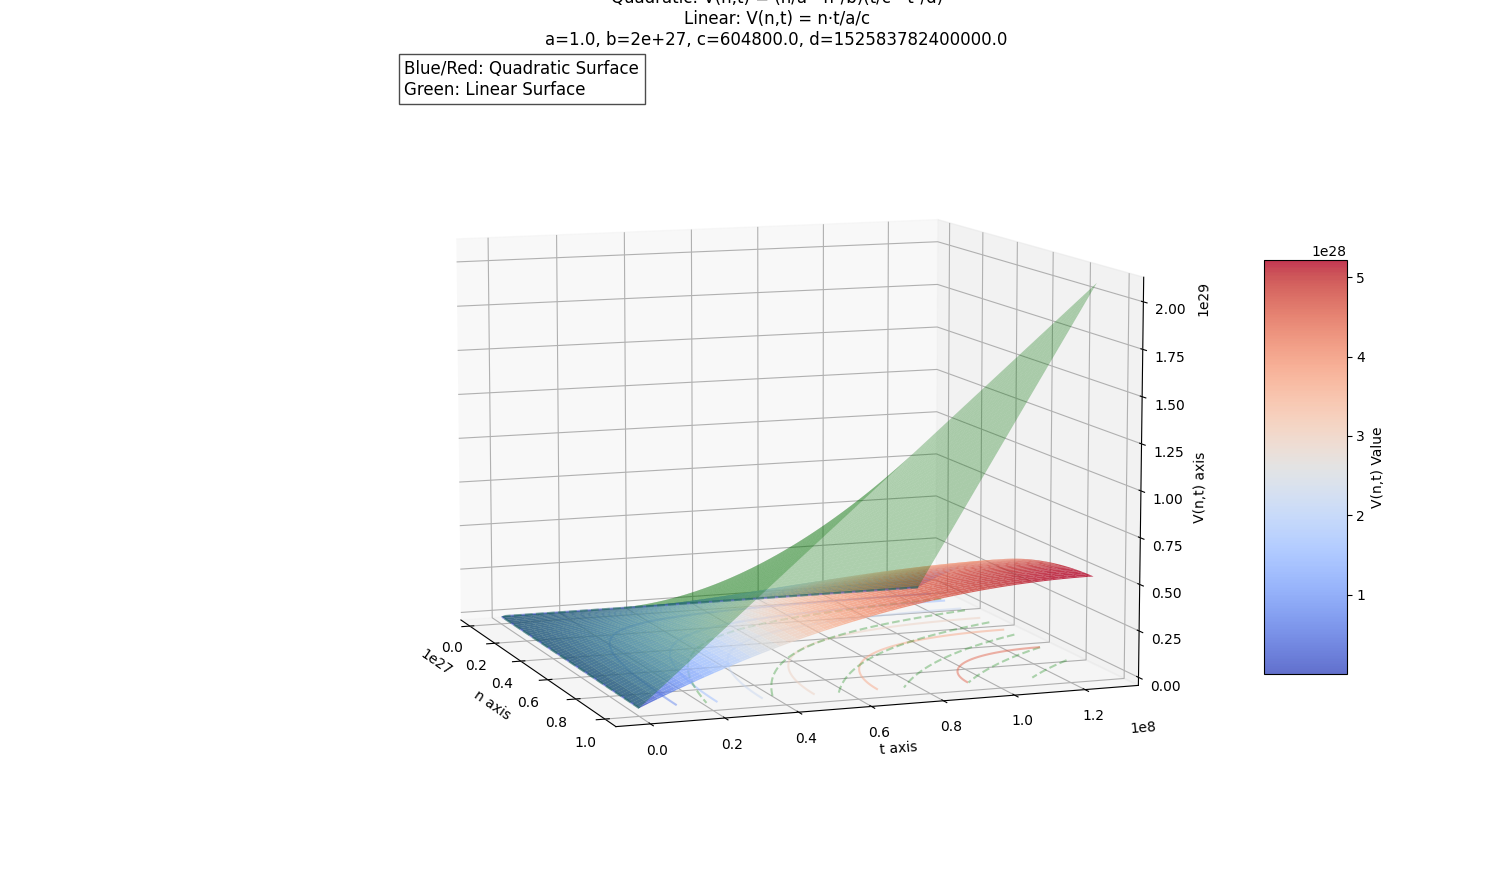
\includegraphics[width=\textwidth]{voting-power-surface.png}
    \caption{An example of $V(n, t)$ compared with the ``linear surface'' $n t / (a b)$.}
    \label{fig:voting-power}
\end{figure}

If $n$ or $t$ is $0$, $V$ is $0$.
The role of the parameters $b$ and $d$ is to make the voting power sub-linear in $n$ and $t$, respectively.
This means that:
\begin{itemize}
    \item A whale who locks a large amount of tokens does not dominate voting to the same degree as they would in the linear case (e.g. if one user owns 51\% of the tokens, locking them all will result in less than 51\% of the possible voting power).
    \item Locking for the maximum period gets less than double locking for half the maximum period.
    \item The sublinearity can be tuned by changing the value of $b$ and $d$.
      As $b$ or $d$ tends to $0$, the voting power tends to linear in $n$ or $t$ respectively.
\end{itemize}

Voting power decreases as time passes.
Say initial lock is for $100~\text{uHYPR}$ for $52~\text{weeks} = 3.14496 \times 10^7~\text{s}$.
Initial voting power is then
\begin{equation}
\begin{aligned}
V(n=100, t=3.14496 \times 10^7) &= (100/a - 100^2/b) \\
	&~~ \cdot (3.14496 \times 10^7~\text{s}\cdot /c - (3.14496 \times 10^7~\text{s})^2/d)
\end{aligned}
\end{equation}

After one week has past, $t$ declines to $51$.
Each subsequent week, voting power of the locked tokens decreases, until it eventually reaches $0$.

A locked token position can be modified in three ways:
\begin{enumerate}
    \item Token lock can be extended.
       For example, say 100 tokens were locked for 52 weeks and 20 have passed, leaving 32 weeks remaining in the lock.
       The user can extend the lock to 52 weeks once again, extending the lockup period by an additional 20 weeks, and bringing voting power up to its original value.
    \item Tokens may be added.
       For example, say 100 tokens we locked for 52 weeks and 20 have passed, leaving 32 weeks remaining in the lock.
       10 additional tokens might be added, leading to a locked set of 110 tokens for 32 weeks.
    \item Tokens within the locked set may be registered, see \hyperref[sec:registration]{Registration discussion below}.
\end{enumerate}

Note that locked tokens are illiquid (cannot be transferred, or interacted with in any way aside from extending lock; adding tokens; registering locked tokens to Hypermap) until the lock time has passed!

\subsection{Deriving $a$, $b$, $c$, $d$}\label{sec:deriving-parameters}

To derive the parameters, we make use of
\begin{enumerate}
	\item Setting $a$ and $c$ such that the smallest unit of $n$ and $t$ yield $1$ voting power,
	\item Using Equation~\ref{eq:parameters-extremum}, derived by setting the partial derivatives of $V(n,t)$ to $0$, to set $b$ and $d$,
	\item Checking that the maximum possible voting power does not exceed the size of a uint256 (of the order of $10^{77}$).
\end{enumerate}

The units of $n$ are uHYPR: the smallest unit of HYPR tokens.
HYPR tokens are divisible into $10^{18}$ uHYPR, and so $a$ is $1$ with units uHYPR.

The units of $t$ are seconds, but the shortest lock time is $1$ week.
Thus we set $c$ to $1$ week of seconds, or $6.048 \times 10^5$ seconds.

Now, to set $b$ and $d$, we use the equalities in Equation~\ref{eq:parameters-extremum}, leading to:
\begin{equation}
\begin{aligned}
b &= 2 a \cdot n_m \\
  &= 2 \times 10^{27}~\text{uHYPR}^2
\end{aligned}
\end{equation}
and
\begin{equation}
\begin{aligned}
d &= 2 c \cdot T \\
  &= 1.525837824 \times 10^{14}~\text{s}^2
\end{aligned}
\end{equation}

Finally, we check if these parameters will lead to a too-large value in the maximum-voting-power case.
The maximum-possible-voting-power case is when $1~\text{uHYPR}$ is held by each of $10^{27}$ wallets, each for the maximum time period of $T$.
This leads to
\begin{equation}
\begin{aligned}
10^{77} & \geq \sum_i^{10^{27}} V(n_i = 1, t = T) \\
	&~~~~= 10^{27} \cdot 1/a \cdot (T/b - T^2/d) \\
\end{aligned}
\end{equation}
where the right-hand side of the equation is much less than the left-hand side: the maximum-voting-power case will easily fit into a uint256.

\section{Registration}\label{sec:registration}

Tokens that are locked can be registered.
Registration can occur on either all locked tokens (that have not yet been registered) or a subset.
Registration points those tokens at a name-key on the Hypermap for some duration: $n_i$, the number of HYPR tokens registered at name-key $i$, and $t_i$, the remaining period tokens are registered for (in weeks) to name-key $i$.\footnote{
	Recall that the Hypermap has two types of keys, name-keys and data-keys.
	Data-keys hold data, whereas name-keys provide hierarchical structure and can be nested.
	Name-keys can have tokens registered to them to indicate value.
	The registration values found on the Hypermap can be used in arbitrarily programmable ways, with current plans to use them for search and filtering.
	More discussion can be found in the \href{https://hyperware.ai/whitepaper.pdf}{Hyperware Whitepaper}.
}
Tokens must be registered for a duration shorter-than-or-equal-to the tokens are locked for $t_i \leq t$.

Offchain applications will determine how to definte registration power for their uses.
A form like voting power is reasonable for some applications, since it will reflect both the user's stake and time horizon.
To take two examples:
\begin{enumerate}
	\item App Store search sorting.
		Devs or others can register tokens to apps in the App Store.
		When a user searches, the total registration power of the app will be used to sort the search results.
		If using a form like voting power, high-value, long-duration apps will appear first.
		This makes sense because it indicates the dev has put a significant stake into the system.
	\item Chat app spam resistance.
		A chat app might have a setting to only allow cold DMs from other users with a certain amount of registration power on their Hyperware node.
		Once again, the idea is that users with more than a certain registration power are invested in the system, and so are unlikely to be bots.
\end{enumerate}

A registered token position on a given name-key can be modified in two ways:
\begin{enumerate}
    \item Token registration can be extended.
       For example, say 100 tokens were registered for 52 weeks and 20 have passed, leaving 32 weeks remaining in the registration.
       The user can extend the registration to 52 weeks once again, extending the registration period by an additional 20 weeks, and bringing registration power up to its original value.
    \item Tokens may be added.
       For example, say 100 tokens we registered for 52 weeks and 20 have passed, leaving 32 weeks remaining in the registration.
       10 additional tokens might be added, leading to a registered set of 110 tokens for 32 weeks.
\end{enumerate}

Note that registered tokens are illiquid (cannot be transferred, or interacted with in any way aside from extending registration or adding tokens) until the registration time has passed!
Note also that token registration positions expire into a locked token position, and can only become truly liquid once the locked token position expires.
For example, say a user has 100 HYPR.
The use locks 80 HYPR for 52 weeks, so now only has 20 HYPR liquid.
Any of the 80 locked HYPR can be registered for up to 52 weeks.
Say 40 is registered to $foo.os$ for 2 weeks and 30 is registered to $app.bar.os$ for 52 weeks.
Then 10 locked HYPR can still be registered at will.
The $foo.os$ registration will expire after 2 weeks, at which time the state of the locked tokens will look like:
\begin{enumerate}
    \item 50 locked and unregistered, free for registration,
    \item 30 registered for 50 weeks.
\end{enumerate}
After an additional 50 weeks, the $app.bar.os$ registration will expire as will the lock, and the tokens can be unlocked and become liquid again.

\begin{table}[htbp]
    \centering
    \caption{Summary of important known and unknown parameters}
    \label{tab:student-performance}
    \begin{tabular}{|c|c|c|}
    \hline
    \textbf{Parameter} & \textbf{Value} & \textbf{Description} \\
    \hline
    $S = n_m$ & $10^9$ & Total token supply \\
    $1$ HYPR & $10^{18}~\text{uHYPR}$ & Each HYPR token has $10^{18}$ ``units'' \\
    $T$ & $4~\text{years} = 208~\text{weeks}$ & Max registration time \\
    $a$ & $1~\text{uHYPR}$ & One uHYPR gives one voting power \\
    $b$ & $2 \times 10^{27}~\text{uHYPR}^2$ & See Section~\ref{sec:deriving-parameters} \\
    $c$ & $6.048 \times 10^5~\text{s}$ & One week gives one voting power \\
    $d$ & $1.525837824 \times 10^{14}~\text{s}^2$ & See Section~\ref{sec:deriving-parameters} \\
    $L_t$ & ? & Lockup duration for team members \\
    $C_t$ & ? & Cliff duration for team members \\
    $L_i$ & ? & Lockup duration for investors \\
    $C_i$ & ? & Cliff duration for investors \\
    \hline
	\end{tabular}
\end{table}

\section{Voting in DAO Governance}\label{sec:voting}

A proposal has a closing time associated with it.
Voters cast votes.
Voting power of voters is calculated at closing time, and the proposal passes or fails.
Voters and their voting power, as well as the result of the vote, is recorded.

\section{Governance Participation Rewards}\label{sec:rewards}

Governance participation incentives are distributed quarterly: 2\% of the remaining incentive treasury per quarter.
For each proposal, $k$, a user $j$ that participates in that vote gets an award $A^{k}_j$ that is a fraction of the incentives dedicated to that vote equal to
\begin{equation}
A^{k}_j = \frac{V^{k}_j}{\sum_j V^{k}_j}
\end{equation}
where $V^{k}_j$ denotes the voting power contributed by user $j$ in the $k$th vote in a quarter.

\begin{figure}[h]
    \centering
    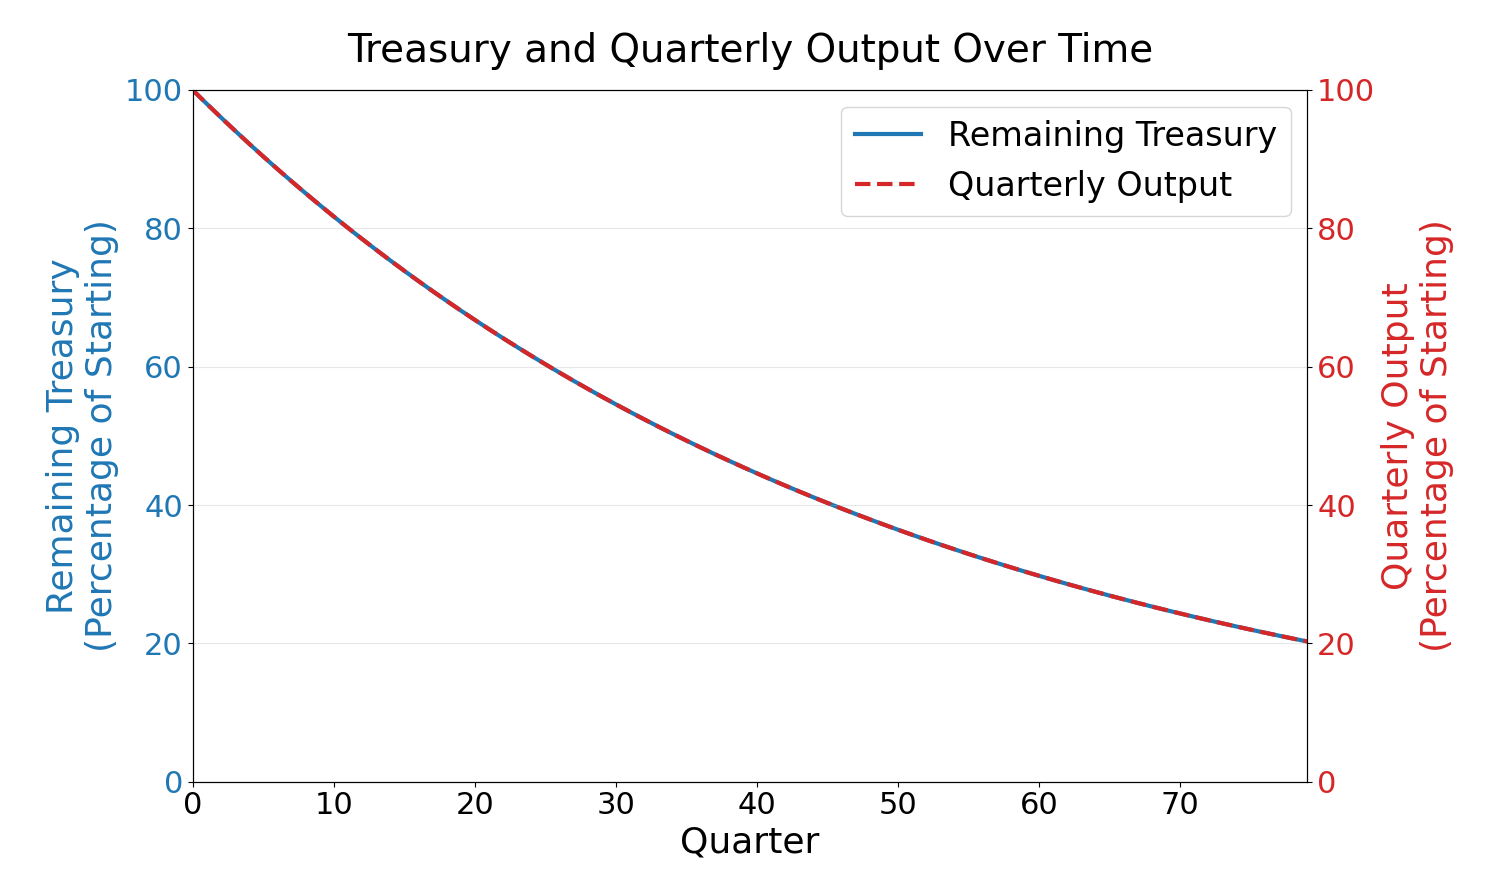
\includegraphics[width=\textwidth]{incentives-treasury-over-time.png}
    \caption{The remaining incentives treasury and quarterly rewards, over time}
    \label{fig:incentives}
\end{figure}

At least one vote will occur each quarter.
If multiple votes occur in a quarter, the incentives are split amongst them based on the total voting power that participated in each vote.
Then the fraction of quarterly incentives allocated to a specific vote $k$, $F^{k}$ is
\begin{equation}
F^{k} = \frac{\sum_j V^{k}_j}{\sum_k \sum_j V^{k}_j}
\end{equation}
and so the total award of a user in a multi-vote quarter becomes
\begin{equation}
A_j = \sum_k \left[F^{k} \cdot A^{k}_j\right]
\end{equation}

Users can delegate their voting power to a third-party.
The delegate's voting power becomes the sum of their own voting power and all voting powers delegated to them
\begin{equation}
V^{(D)}_i = V_i + \sum_j V_j
\end{equation}
Incentive rewards are distributed to the owners of the voting powers, not the delegate.
If the delegate does not cast a vote, the voting power delegated to them earns no rewards from that vote.

\section{Vesting}\label{sec:vesting}

Vesting tokens cannot do anything except have the vested fraction claimed, depending on the percentage of the vesting time that has passed.
Thus, they cannot participate in locking, registration, or governance.
They cannot be transferred.

There are two reasons that vesting tokens cannot participate in registration or governance:
\begin{enumerate}
    \item Simplicity.
         Vesting tokens will only exist for the start of the network.
         There should not be logic for them that lives forever in locking, governance, registration contracts.
    \item Giving community members a headstart on governance and incentive rewards.
         Investors and team members will only be able to access a fraction of their tokens -- the ones that have already vested -- and thus will not be able to control governance due to their outsized ownership in early days.
         This also gives community members a chance to acquire a larger fraction of the governance rewards, improving the distribution of tokens to the community.
         Investors and team members have been of fundamental importance to the project and will continue to be so, but establishing an involved and aligned community is of the utmost importance for Hyperware to succeed.
\end{enumerate}

\end{document}
